\begin{tiny}(Ccp41)\end{tiny} On cherche à montrer qu'il existe un unique $u$ réel tel que
\begin{displaymath}
  \left|z-u\right|^2 = \left|w-u\right|^2.
\end{displaymath}
Ceci est en fait une équation du premier degré en $u$ car les $|u|^2$ se simplifient en développant. On obtient donc une unique solution
\begin{displaymath}
  u = 
  \frac{|z|^2-|w|^2}{2\left( \Re(z) - \Re(w)\right) }
\end{displaymath}
\begin{figure}
  \centering
  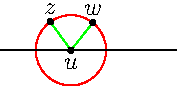
\includegraphics{./Ccp41_1.pdf}
  % Ccp41_1.pdf: 0x0 pixel, -2147483648dpi, 0.00x0.00 cm, bb=
  \caption{Exercice \ref{Ecp41}}
  \label{fig: Ccp41_1}
\end{figure}

